\section{Model fitting} \label{sec:ModelFitting}
In the following section we try to find and determine a model to describe the evolution of the done status of the nodes in function of the time passed, given the shape shown in Figure \ref{fig:done-status} there are several options that fit the general trend of the curve:

\begin{itemize}
	\item Logistic model $ Y = \frac{A}{1 + e^{-rt}} $
	\item Gompertz model $ Y = Ae^{-Be^{-rt}} $
	\item Sigmoid model $ Y = A\frac{1-e^{-rt}}{1+e^{-rt}}$
	\item Asymptotic model $ Y = A + Be^{-rt}$
\end{itemize} 

The next step is to find the most adapt for our case, by looking for the requirement and assumption of each model some of them need to be excluded. The first one is quickly discarded because it requires the output to have only two possible outcomes, such as "success" and "failure", this is not the case.
Similarly the Sigmoid model is discard because it assume the output to follow a S shape behavior with a slow start,an accelerated growth and then a slow decline, depending on the configuration for the runs this is not always true.


The requirements for both Gompertz and asymptotic models are met, in particular:
\begin{itemize}
	\item the outcome variable is continuous
	\item there is no multicollinearity
	\item the sample is large enough
	\item there are no outliers
	\item the linearity of the logarithm is respected
	
	\item for the Gomperz
		\begin{itemize}
			\item the sample shows a monotonic behavior
		\end{itemize}
		\item for the asymptotic
		\begin{itemize}
			\item the sample shows a asymptotic behavior
		\end{itemize}
\end{itemize}

By performing a residual analysis the Gomperz model result to be the most suited for our samples, it also fits the logic of one of its typical usage of examining disease spread. Following there is the QQ plot between the theoretical distribution on the X axis and the sample one in the Y axis.

\begin{figure}[H]
\centering
    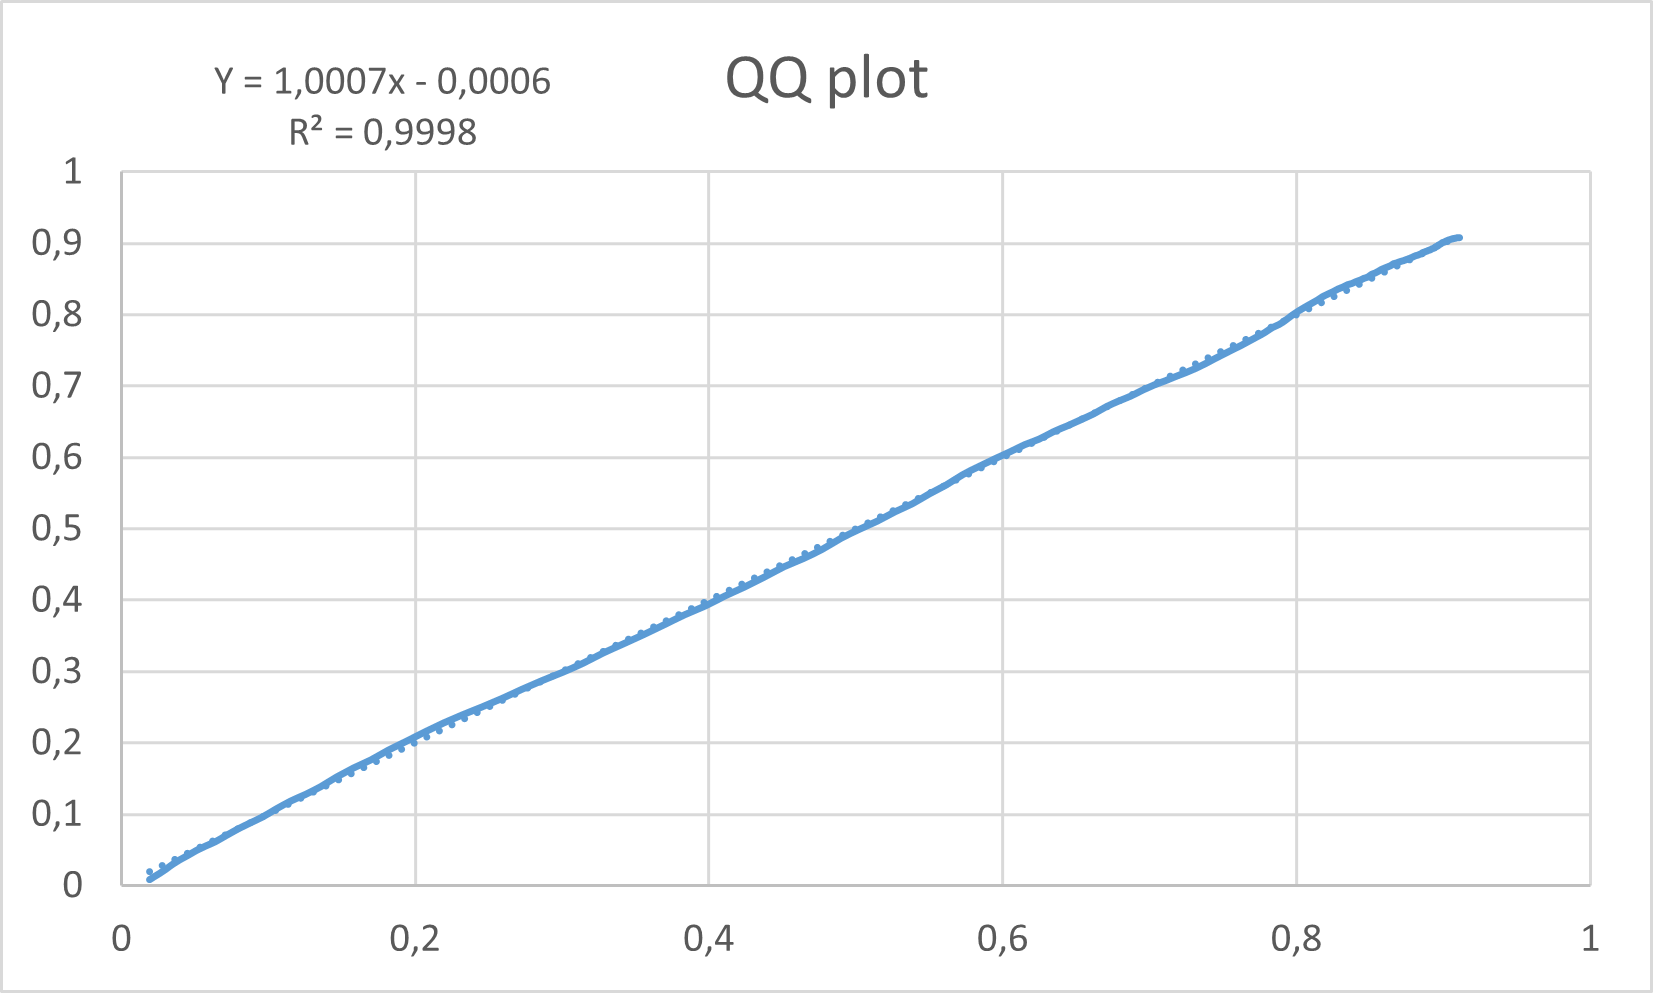
\includegraphics[width= 1\textwidth]{./images/QQPlot200.png}
\end{figure}

It is clear that there is a linear relationship between the values from our sample and the ones from the Gompertz model, this is also indicated by the value for $R^2$.

\section{Factorial analysis on the models parameters}
As previously stated we consider for extremes the values 0.15 and 0.85 for probability and 10 and 75 for the range.

The Gompertz model ($ Y = Ae^{-Be^{-rt}} $) has three parameters:
\begin{itemize}
	\item A is the asymptote
	\item B is the displacement on the x axis
	\item r is the grow rate
\end{itemize}
The first to be analyzed is the asymptote.


\begin{table}[H]
\centering
\begin{tabular}{|cl|ll|l}
\cline{1-4}
\multicolumn{2}{|c|}{\multirow{2}{*}{Asymptote}}        & \multicolumn{2}{c|}{Radius}              &  \\ \cline{3-4}
\multicolumn{2}{|c|}{}                                  & \multicolumn{1}{l|}{10}       & 75       &  \\ \cline{1-4}
\multicolumn{1}{|c|}{\multirow{2}{*}{Probability}} & 0.15 & \multicolumn{1}{l|}{0,911651} & 0,999465 &  \\ \cline{2-4}
\multicolumn{1}{|c|}{}                             & 0.85 & \multicolumn{1}{l|}{0,574134} & 0,918475 &  \\ \cline{1-4}
\end{tabular}
\caption{Extreme factor levels for asymptote}
\end{table}


\begin{table}[H]
\centering
\begin{tabular}{l|l|l|l|l|ll}
\cline{2-7}
 & I & Prob & Radius & RP & \multicolumn{1}{l|}{Asymptote} & \multicolumn{1}{l|}{SST\_i} \\ \cline{2-7} 
 & 1 & -1 & -1 & 1 & \multicolumn{1}{l|}{0,911651} & \multicolumn{1}{l|}{0,003687} \\ \cline{2-7} 
 & 1 & 1 & -1 & -1 & \multicolumn{1}{l|}{0,574134} & \multicolumn{1}{l|}{0,076617} \\ \cline{2-7} 
 & 1 & -1 & 1 & -1 & \multicolumn{1}{l|}{0,999465} & \multicolumn{1}{l|}{0,022062} \\ \cline{2-7} 
 & 1 & 1 & 1 & 1 & \multicolumn{1}{l|}{0,918475} & \multicolumn{1}{l|}{0,004562} \\ \hline
\multicolumn{1}{|l|}{4q} & 3,403726 & -0,41851 & 0,432155 & 0,256526 & \multicolumn{1}{l|}{Total} & \multicolumn{1}{l|}{0,106928} \\ \hline
\multicolumn{1}{|l|}{q} & 0,850931 & -0,10463 & 0,108039 & 0,064132 &  &  \\ \cline{1-5}
\multicolumn{1}{|l|}{4 q\textasciicircum{}2} &  & 0,043787 & 0,046689 & 0,016451 &  &  \\ \cline{1-5}
\multicolumn{1}{|l|}{Influence} &  & 0,409502 & 0,436643 & 0,153855 &  &  \\ \cline{1-5}
\end{tabular}
\caption{Influence of factors for asymptote}
\end{table}

We then follow with the tables for displacement.

\begin{table}[H]
\centering
\begin{tabular}{|cl|ll|}
\hline
\multicolumn{2}{|c|}{\multirow{2}{*}{Displacement}} & \multicolumn{2}{c|}{Radius} \\ \cline{3-4} 
\multicolumn{2}{|c|}{} & \multicolumn{1}{l|}{10} & 75 \\ \hline
\multicolumn{1}{|c|}{\multirow{2}{*}{Probability}} & 15 & \multicolumn{1}{l|}{4,095867} & 1,862222 \\ \cline{2-4} 
\multicolumn{1}{|c|}{} & 85 & \multicolumn{1}{l|}{3,869347} & 0,590452 \\ \hline
\end{tabular}
\caption{Extreme factor levels for displacement}
\end{table}


\begin{table}[H] \label{tab:Displacement}
\centering
\begin{tabular}{l|l|l|l|l|ll}
\cline{2-7}
 & I & Prob & Radius & RP & \multicolumn{1}{l|}{Displacement} & \multicolumn{1}{l|}{SS\_i} \\ \cline{2-7} 
 & 1 & -1 & -1 & 1 & \multicolumn{1}{l|}{4,095867} & \multicolumn{1}{l|}{2,224258} \\ \cline{2-7} 
 & 1 & 1 & -1 & -1 & \multicolumn{1}{l|}{3,869347} & \multicolumn{1}{l|}{1,599909} \\ \cline{2-7} 
 & 1 & -1 & 1 & -1 & \multicolumn{1}{l|}{1,862222} & \multicolumn{1}{l|}{0,550935} \\ \cline{2-7} 
 & 1 & 1 & 1 & 1 & \multicolumn{1}{l|}{0,590452} & \multicolumn{1}{l|}{4,056277} \\ \hline \multicolumn{1}{|l|}{4q} & 10,41789 & -1,49829 & -5,51254 & -1,04525 & \multicolumn{1}{l|}{Total:} & \multicolumn{1}{l|}{8,431378} \\ \hline
\multicolumn{1}{|l|}{q} & 2,604472 & -0,37457 & -1,37813 & -0,26131 &  &  \\ \cline{1-5}
\multicolumn{1}{|l|}{4 q\textasciicircum{}2} &  & 0,561218 & 7,597023 & 0,273137 &  &  \\ \cline{1-5}
\multicolumn{1}{|l|}{Influenza} &  & 0,066563 & 0,901042 & 0,032395 &  &  \\ \cline{1-5}
\end{tabular}
\caption{Influence of factors for displacement}
\end{table}

Finally we end up with the tables for the growth rate.

\begin{table}[H]
\centering
\begin{tabular}{|cl|ll|}
\hline
\multicolumn{2}{|c|}{\multirow{2}{*}{Growth Rate}} & \multicolumn{2}{c|}{Radius} \\ \cline{3-4} 
\multicolumn{2}{|c|}{} & \multicolumn{1}{l|}{10} & 75 \\ \hline
\multicolumn{1}{|c|}{\multirow{2}{*}{Probability}} & 15 & \multicolumn{1}{l|}{0,04144} & 0,128276 \\ \cline{2-4} 
\multicolumn{1}{|c|}{} & 85 & \multicolumn{1}{l|}{0,159516} & 0,366016 \\ \hline
\end{tabular}
\caption{Extreme factor levels for growth rate}
\end{table}

\begin{table}[H]
\centering
\begin{tabular}{l|l|l|l|l|ll}
\cline{2-7}
 & I & Prob & Radius & RP & \multicolumn{1}{l|}{Growth rate} & \multicolumn{1}{l|}{SS\_i} \\ \cline{2-7} 
 & 1 & -1 & -1 & 1 & \multicolumn{1}{l|}{0,04144} & \multicolumn{1}{l|}{0,017522} \\ \cline{2-7} 
 & 1 & 1 & -1 & -1 & \multicolumn{1}{l|}{0,159516} & \multicolumn{1}{l|}{0,000204} \\ \cline{2-7} 
 & 1 & -1 & 1 & -1 & \multicolumn{1}{l|}{0,128276} & \multicolumn{1}{l|}{0,002074} \\ \cline{2-7} 
 & 1 & 1 & 1 & 1 & \multicolumn{1}{l|}{0,366016} & \multicolumn{1}{l|}{0,036943} \\ \hline
\multicolumn{1}{|l|}{4q} & 0,695249 & 0,355816 & 0,293337 & 0,119664 & \multicolumn{1}{l|}{Total} & \multicolumn{1}{l|}{0,056743} \\ \hline
\multicolumn{1}{|l|}{q} & 0,173812 & 0,088954 & 0,073334 & 0,029916 &  &  \\ \cline{1-5}
\multicolumn{1}{|l|}{4 q\textasciicircum{}2} &  & 0,031651 & 0,021512 & 0,00358 &  &  \\ \cline{1-5}
\multicolumn{1}{|l|}{Influenza} &  & 0,557802 & 0,379108 & 0,06309 &  &  \\ \cline{1-5}
\end{tabular}
\caption{Influence of factors for growth rate}
\end{table}

These results confirm our initial ideas and expectations, the first thing to notice is the influences for the asymptote are similar to the ones for the coverage percentage; this make sense because the asymptote is the maximum reach of the curve and the coverage percentage is the maximum coverage that a run achieves, so it's natural for them to be almost the same. 

\medskip
The displacement represent how high is the rate for nodes in the done status at the second clock of each run, the first one is excluded because it's always constant due to the fact that at the first clock only the zero-patient node is done. By translating these results on the actual model for the analysis the displacement represent how well is connected the firstly infected node and how many of its neighbor immediately pass the check for sending a new infection message. It make sense for the radius to have 90\% influence because having a big radius means having a lot of neighbor. Pay attention that the q values in \ref{tab:Displacement} are negative so, by incrementing the radius, we are diminishing the displacement; this makes sense since lower values for the B parameter indicates a higher Y(t) when t = 0 in the Gompertz function. A low displacement is not always a good thing however because a big radius, as previously shown, can lead to more collision and less coverage percentage in some cases. 

\medskip
The growth rate, as its name suggests, indicates how much fast the curve in grows. In regards of the analysis a high growth rate is achieved when nodes do not experience many collisions and, after receiving a message correctly, can quickly transmit which translate to quickly passing the lottery. So it make sense for the probability to influence the 55\% of the result. The radius accounts for a little more the a third of the influence this is easy to imagine since a high radius means a high number of nodes reached.

\medskip
These results give us an general idea on how the factor weight on the model and how to maximize certain aspect of it, but to perform a proper analysis of the system it is a good idea to pair these values with the box-plot and factorial analysis previously presented.